\section{Présentation des fenêtres}

\subsection{IHM client}

L'IHM Client va permettre de consulter les informations sur le Client.
Elle est appelée à partir de recherche sur un client spécifique. Où à partir d'un lien vers un contact.


\begin{center}
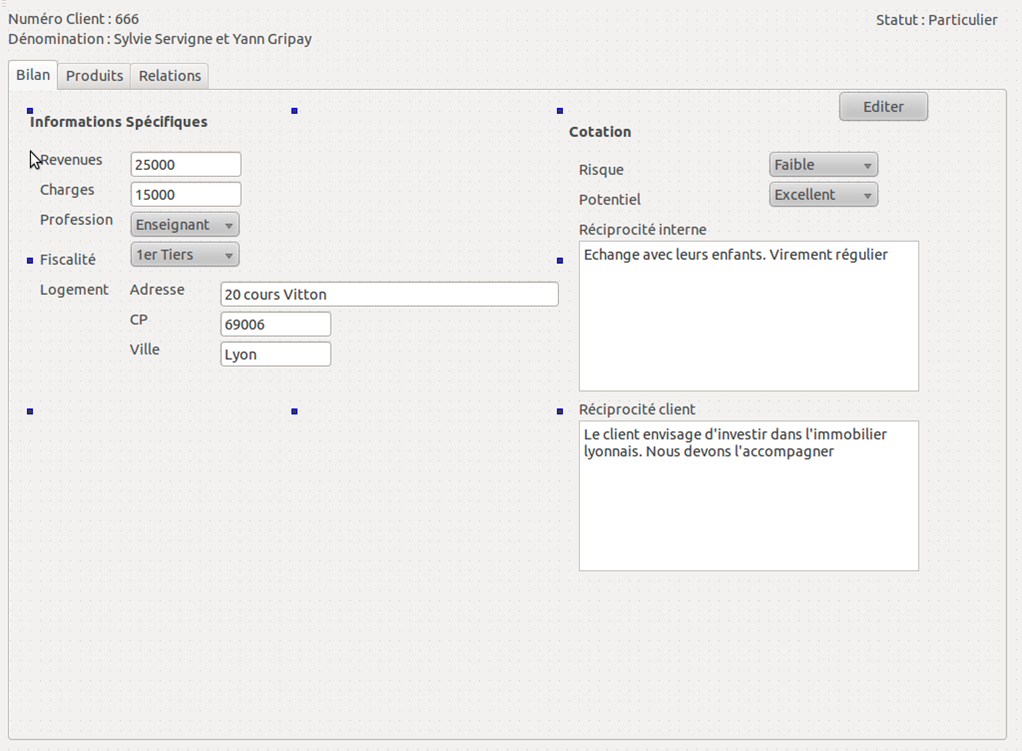
\includegraphics[width=10cm]{\PIXPATH/client1}
\end{center}
\begin{center}
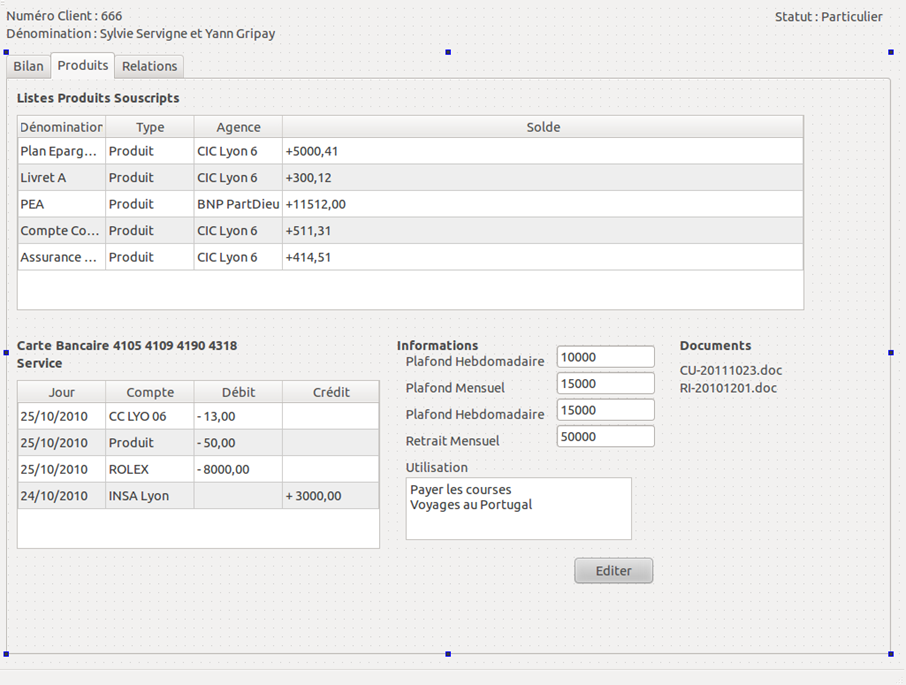
\includegraphics[width=10cm]{\PIXPATH/client2}
\end{center}
\begin{center}
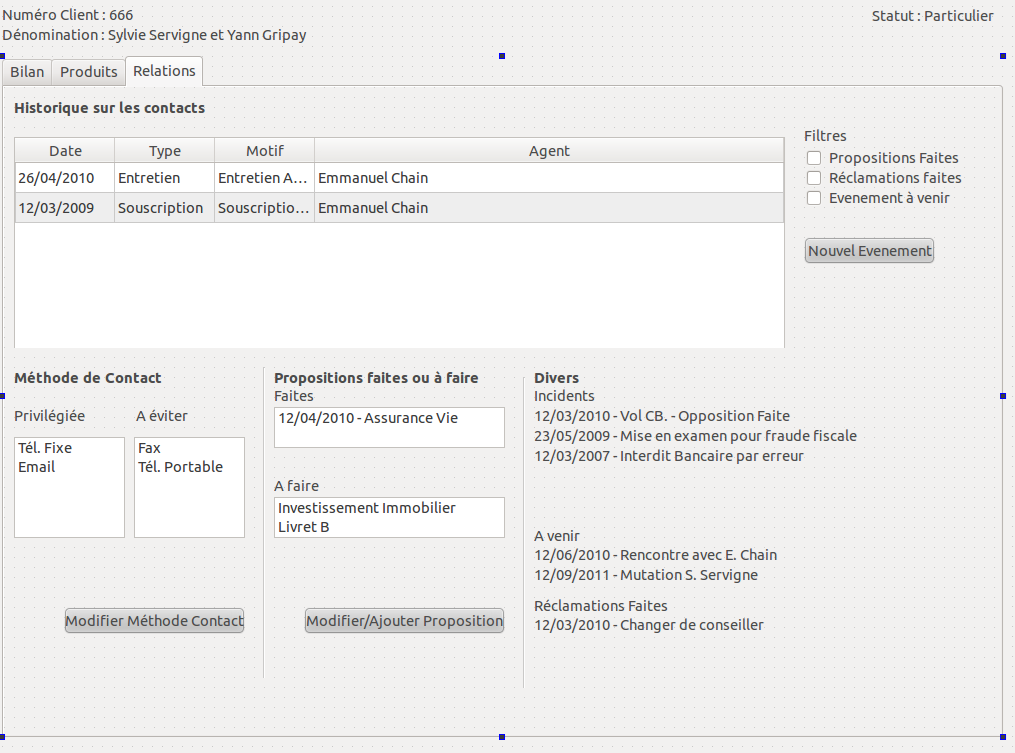
\includegraphics[width=10cm]{\PIXPATH/client3}
\end{center}

\subsection{IHM Agenda}

L'IHM Agenda permet à un agent de consulter son agenda, mais également
celui des autres. En plus de la consultation, il est également possible
de gérer (créer, annuler, déplacer, réaffecter) les rendez-vous des
agents de l'agence.

Deux vues sont possibles: une vue par semaine, pour un seul agent; ou
une vue par jour, affichant tous les agents.

Le chef d'agence peut accéder à un mode «planification» qui lui permet
d'affecter des tâches à ses agents. Ce mode est disponible pour les
deux types de vues.
\begin{center}
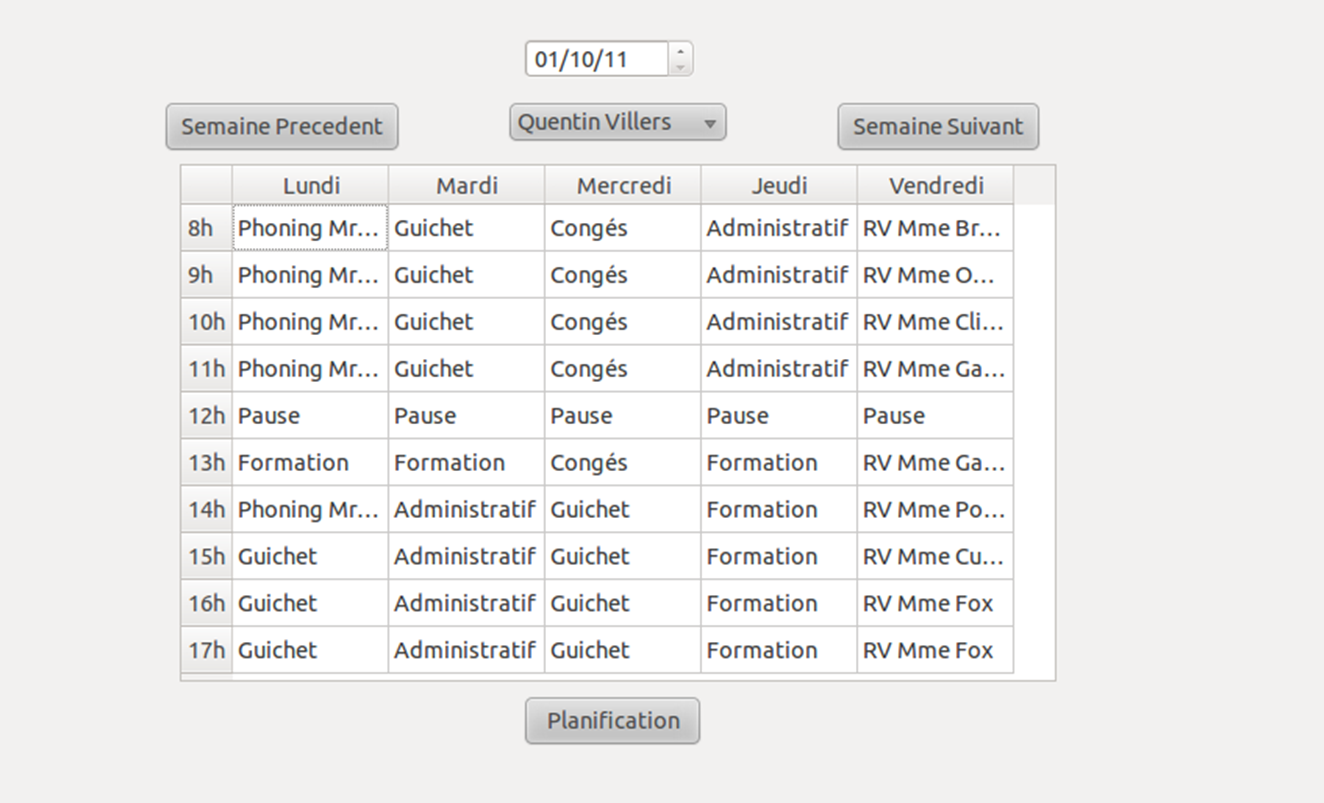
\includegraphics[width=10cm]{\PIXPATH/agenda1}
\end{center}

\begin{center}
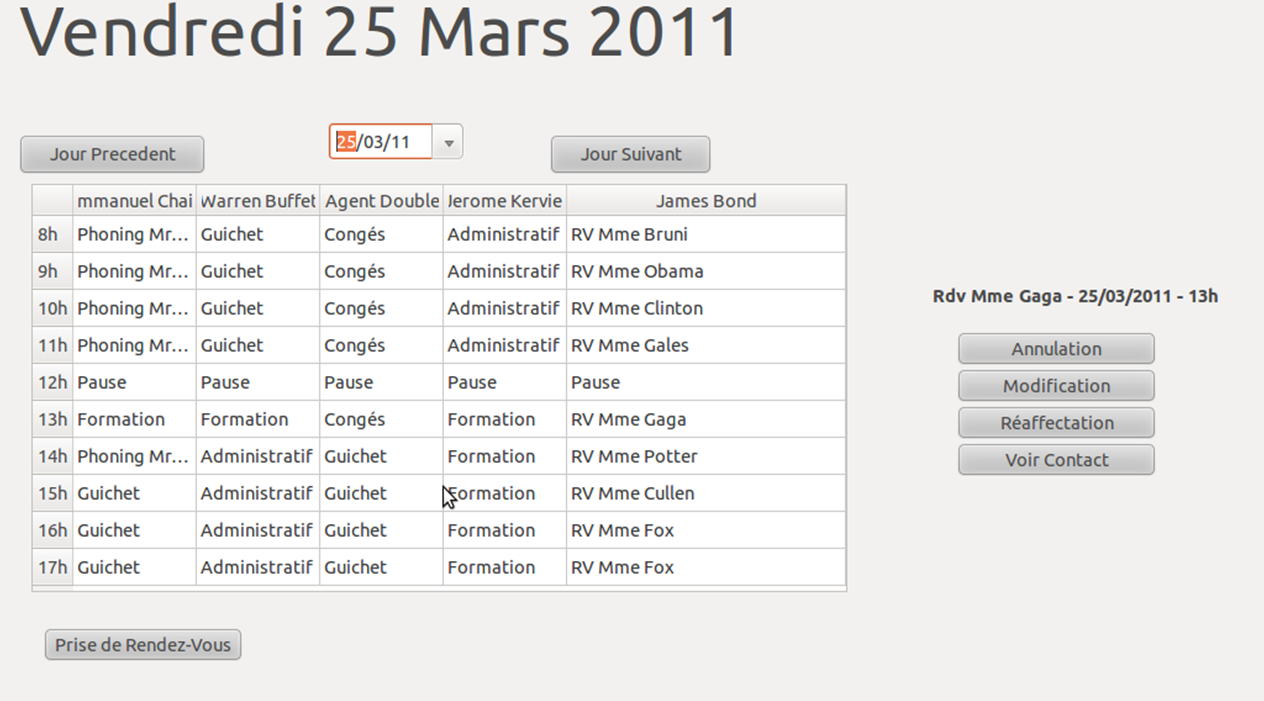
\includegraphics[width=10cm]{\PIXPATH/agenda2}
\end{center}

\subsection{IHM Contact}

L'IHM Contact va permettre à l'agent de préparer un compte-rendu de préparation
d'entretien et rédiger le RAC.

\begin{center}
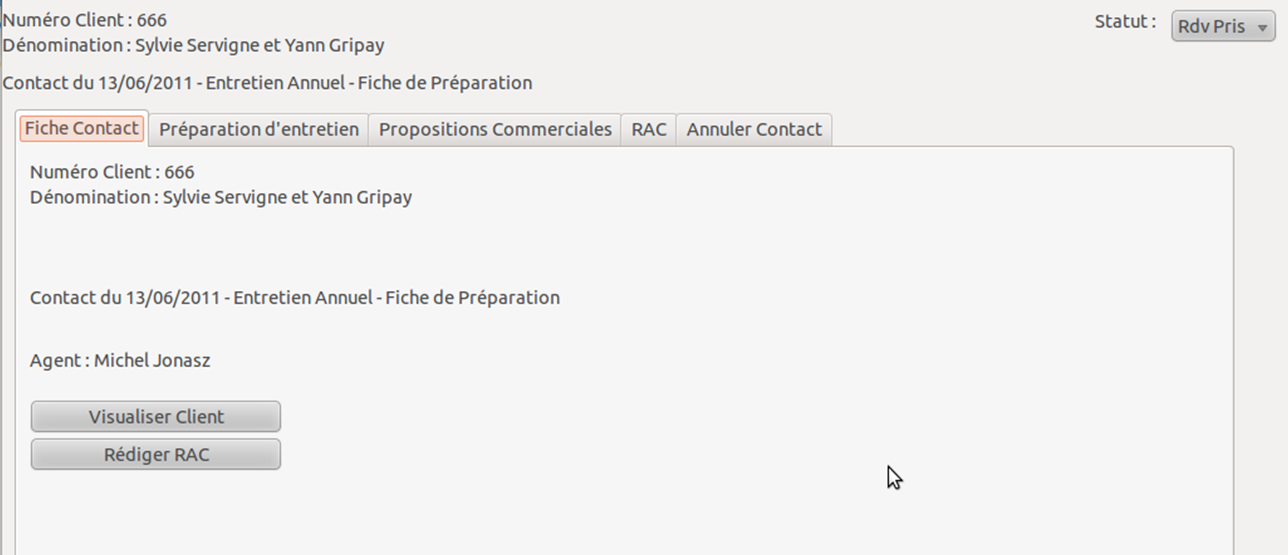
\includegraphics[width=10cm]{\PIXPATH/contact1}
\end{center}
\begin{center}
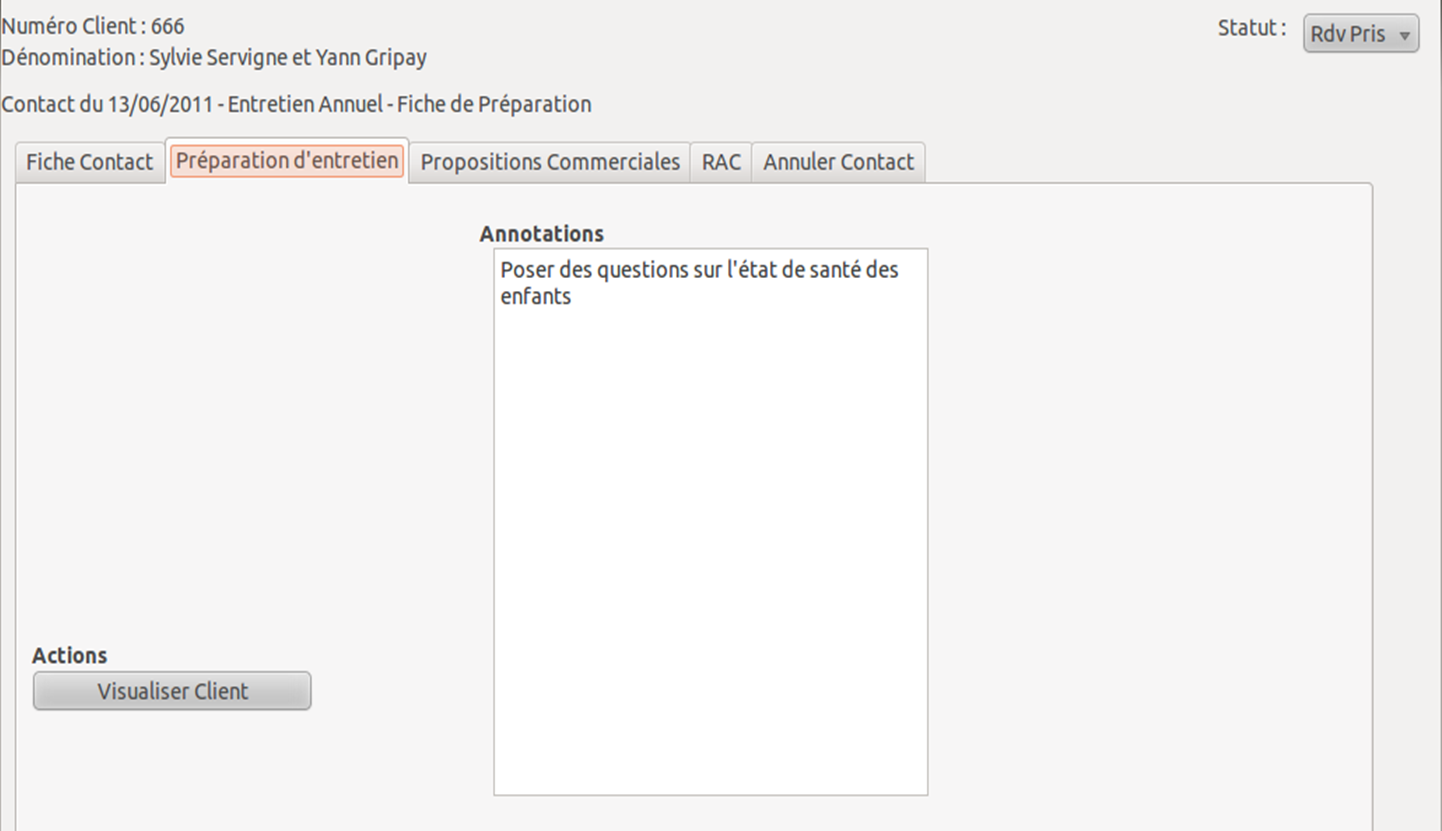
\includegraphics[width=10cm]{\PIXPATH/contact2}
\end{center}
\begin{center}
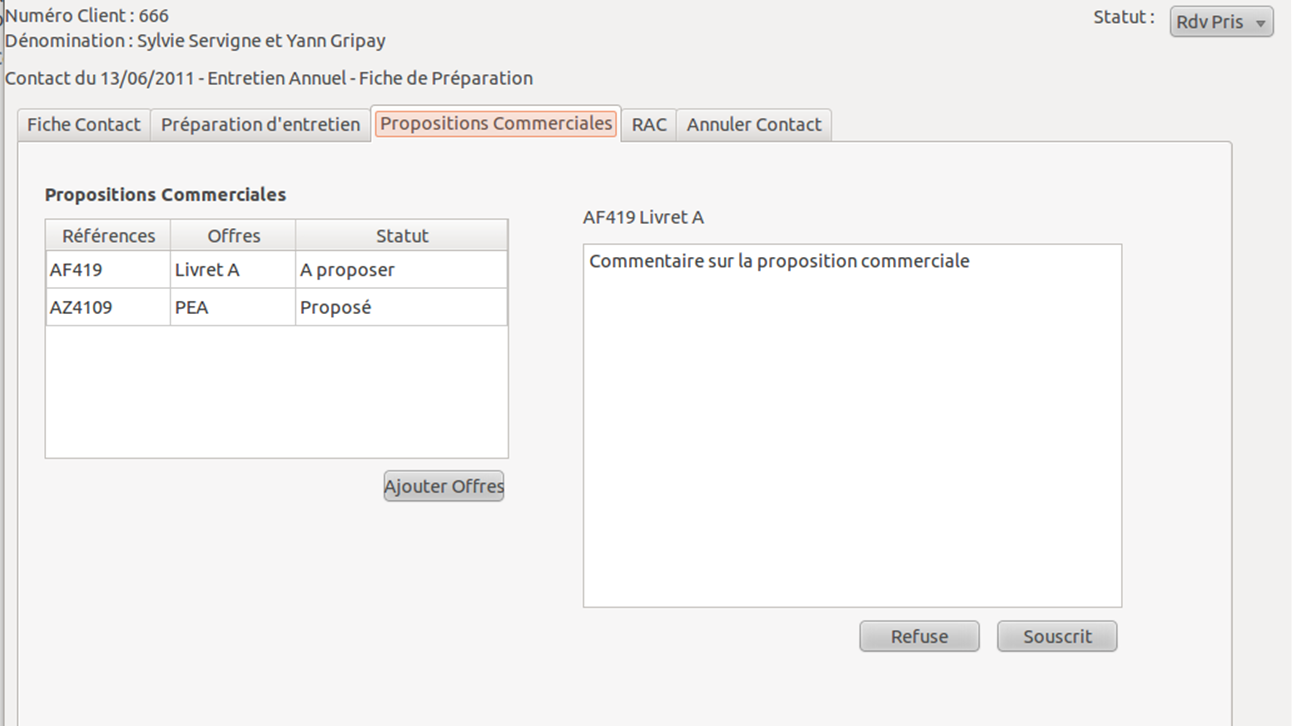
\includegraphics[width=10cm]{\PIXPATH/contact3}
\end{center}
\begin{center}
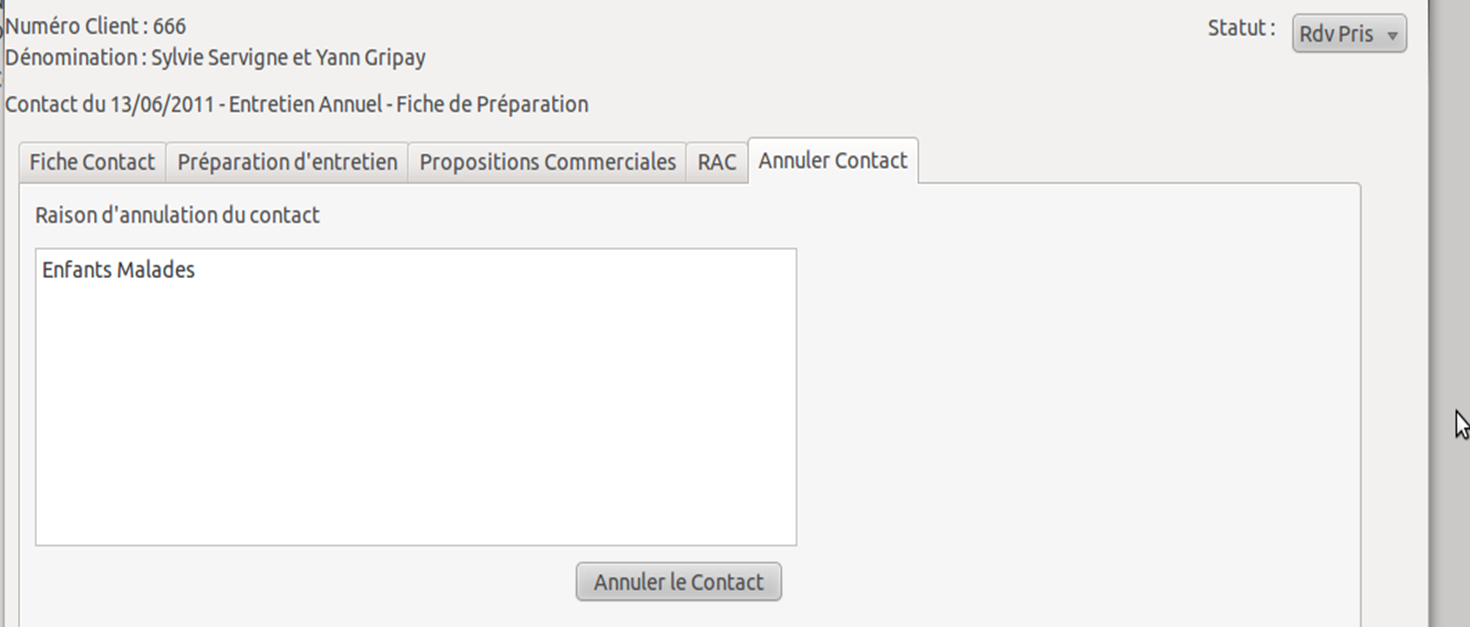
\includegraphics[width=10cm]{\PIXPATH/contact4}
\end{center}

\subsection{IHM Agence}

L'IHM Agence permet de consulter les agents dans une agence et des informations 
de base sur l'agence. Sélectionner un agent permet d'accéder aux informations 
de l'agent, dont sa liste de client et son planning. Il y a par ailleurs la vue 
du chef d'agence qui permet d'accéder à la planification mensuelle de l'agence 
et d'affecter des contacts à des agents. 

\begin{center}
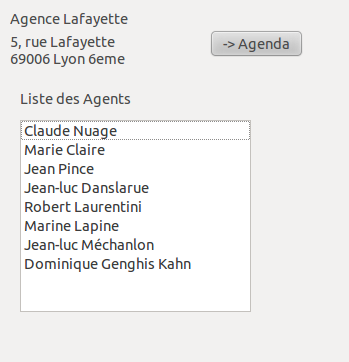
\includegraphics[width=10cm]{\PIXPATH/agence1}
\end{center}
\begin{center}
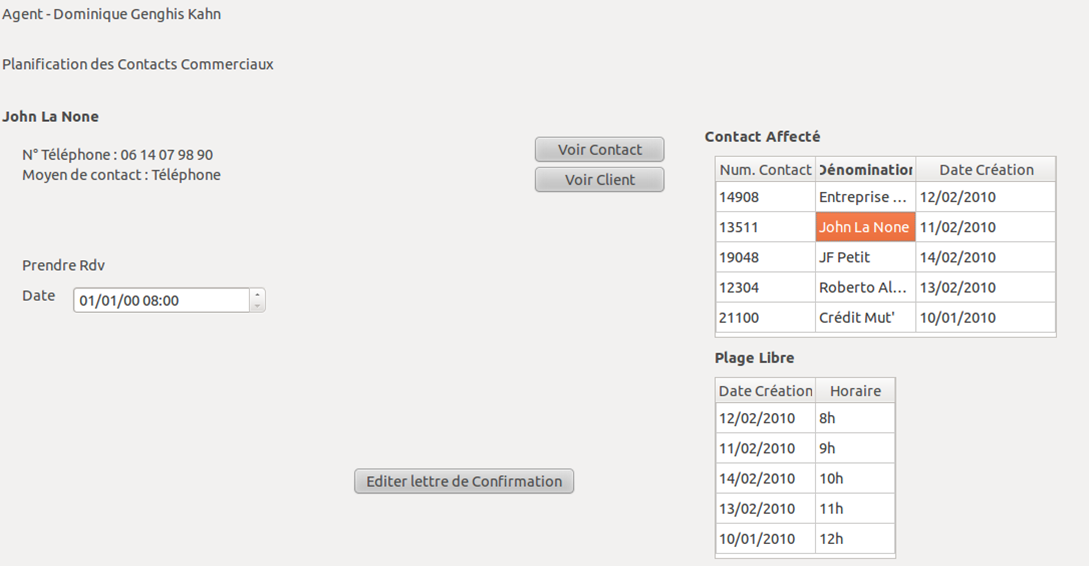
\includegraphics[width=10cm]{\PIXPATH/agence2}
\end{center}
\begin{center}
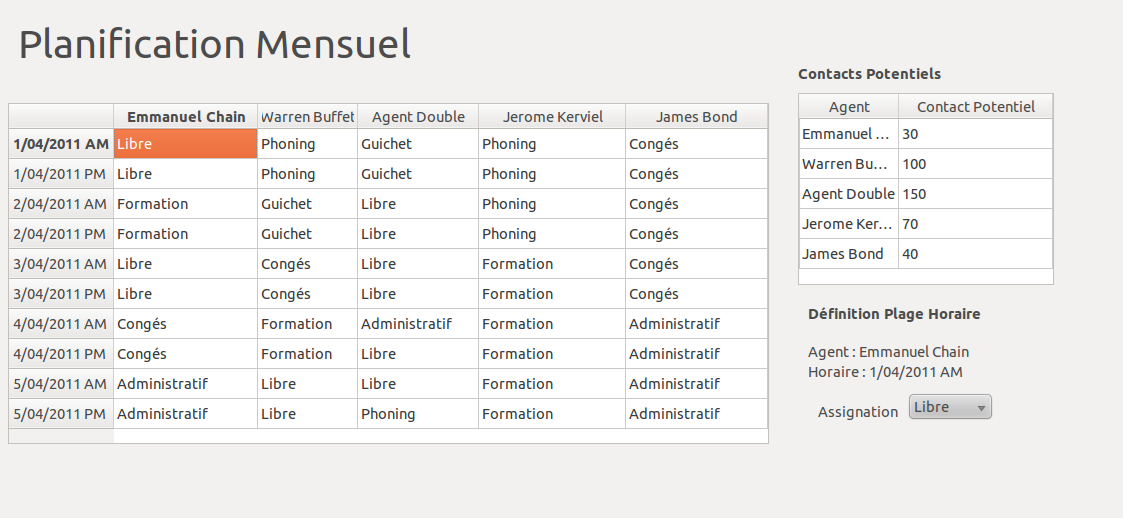
\includegraphics[width=10cm]{\PIXPATH/chef1}
\end{center}
\begin{center}
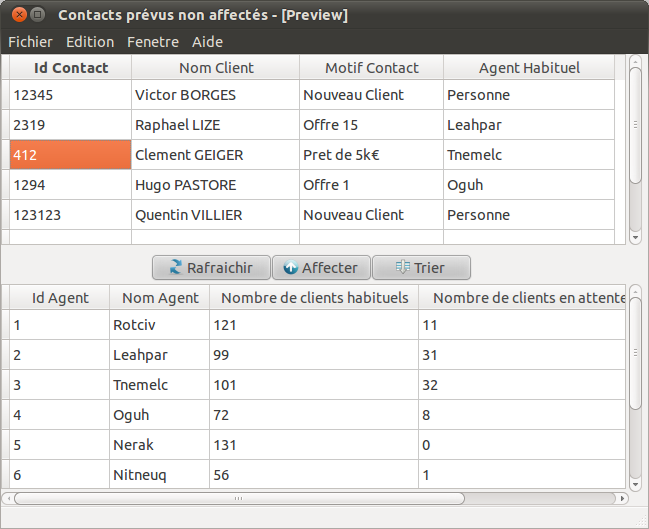
\includegraphics[width=10cm]{\PIXPATH/chef2}
\end{center}

% \subsection{IHM Évènement}
% L'IHM Évènements va permettre de consulter la liste des évènements arrivés
% durant la journée, de générer les motifs de contact correspondants puis les
% contacts prévus.\\

% À chaque étape (évènements, motifs de contact et contacts prévus), la liste
% des objets concernés est visible et chaque objet peut être :
% \begin{itemize}
% \item Visualisé en détail
% \item Édité
% \item Supprimé
% \end{itemize}

% \begin{center}
% 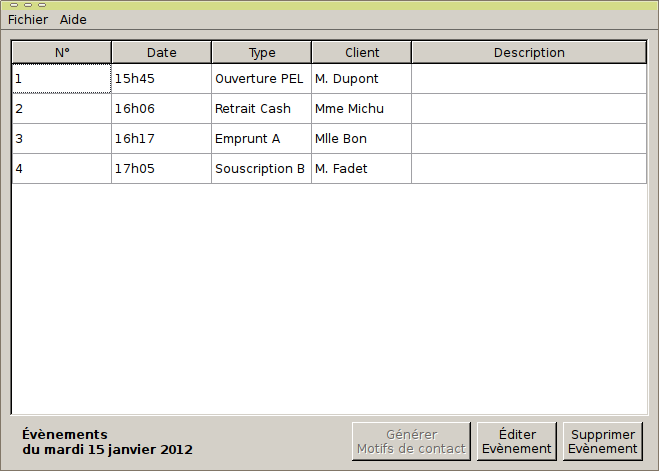
\includegraphics[width=10cm]{\PIXPATH/event1}
% \end{center}
% \begin{center}
% 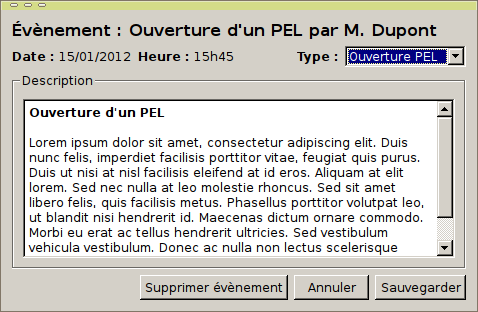
\includegraphics[width=10cm]{\PIXPATH/event2}
% \end{center}
